\documentclass[portrait,final,a0paper]{baposter}
%\documentclass[a4shrink,portrait,final]{baposter}
% Usa a4shrink for an a4 sized paper.

\tracingstats=2

\usepackage{calc}
\usepackage{graphicx}
\usepackage{amsmath}
\usepackage{amssymb}
\usepackage{relsize}
\usepackage{multirow}
\usepackage{bm}

\usepackage{graphicx}
\usepackage{multicol}

\usepackage{pgfbaselayers}
\pgfdeclarelayer{background}
\pgfdeclarelayer{foreground}
\pgfsetlayers{background,main,foreground}

\usepackage{times}
\usepackage{helvet}
%\usepackage{bookman}
\usepackage{palatino}

% i added
\usepackage{epstopdf}
\usepackage{multirow}
%%%%% my add-ons %%%%%
\newcommand{\vect}[1]{\boldsymbol{#1}}
\newcommand{\T}{\texttt}
%%%%%%%%%%%%%%%%%%%%%%

\newcommand{\captionfont}{\footnotesize}

\selectcolormodel{cmyk}

\graphicspath{{images/}}

%%%%%%%%%%%%%%%%%%%%%%%%%%%%%%%%%%%%%%%%%%%%%%%%%%%%%%%%%%%%%%%%%%%%%%%%%%%%%%%%
%%%% Some math symbols used in the text
%%%%%%%%%%%%%%%%%%%%%%%%%%%%%%%%%%%%%%%%%%%%%%%%%%%%%%%%%%%%%%%%%%%%%%%%%%%%%%%%
% Format 
\newcommand{\Matrix}[1]{\begin{bmatrix} #1 \end{bmatrix}}
\newcommand{\Vector}[1]{\Matrix{#1}}
\newcommand*{\SET}[1]  {\ensuremath{\mathcal{#1}}}
\newcommand*{\MAT}[1]  {\ensuremath{\mathbf{#1}}}
\newcommand*{\VEC}[1]  {\ensuremath{\bm{#1}}}
\newcommand*{\CONST}[1]{\ensuremath{\mathit{#1}}}
\newcommand*{\norm}[1]{\mathopen\| #1 \mathclose\|}% use instead of $\|x\|$
\newcommand*{\abs}[1]{\mathopen| #1 \mathclose|}% use instead of $\|x\|$
\newcommand*{\absLR}[1]{\left| #1 \right|}% use instead of $\|x\|$

\def\norm#1{\mathopen\| #1 \mathclose\|}% use instead of $\|x\|$
\newcommand{\normLR}[1]{\left\| #1 \right\|}% use instead of $\|x\|$

%%%%%%%%%%%%%%%%%%%%%%%%%%%%%%%%%%%%%%%%%%%%%%%%%%%%%%%%%%%%%%%%%%%%%%%%%%%%%%%%
% Multicol Settings
%%%%%%%%%%%%%%%%%%%%%%%%%%%%%%%%%%%%%%%%%%%%%%%%%%%%%%%%%%%%%%%%%%%%%%%%%%%%%%%%
\setlength{\columnsep}{0.7em} % 0.7em
\setlength{\columnseprule}{0mm}


%%%%%%%%%%%%%%%%%%%%%%%%%%%%%%%%%%%%%%%%%%%%%%%%%%%%%%%%%%%%%%%%%%%%%%%%%%%%%%%%
% Save space in lists. Use this after the opening of the list
%%%%%%%%%%%%%%%%%%%%%%%%%%%%%%%%%%%%%%%%%%%%%%%%%%%%%%%%%%%%%%%%%%%%%%%%%%%%%%%%
\newcommand{\compresslist}{%
\setlength{\itemsep}{1pt}%
\setlength{\parskip}{0pt}%
\setlength{\parsep}{0pt}%
}


%%%%%%%%%%%%%%%%%%%%%%%%%%%%%%%%%%%%%%%%%%%%%%%%%%%%%%%%%%%%%%%%%%%%%%%%%%%%%%
%%% Begin of Document
%%%%%%%%%%%%%%%%%%%%%%%%%%%%%%%%%%%%%%%%%%%%%%%%%%%%%%%%%%%%%%%%%%%%%%%%%%%%%%

\begin{document}

%%%%%%%%%%%%%%%%%%%%%%%%%%%%%%%%%%%%%%%%%%%%%%%%%%%%%%%%%%%%%%%%%%%%%%%%%%%%%%
%%% Here starts the poster
%%%---------------------------------------------------------------------------
%%% Format it to your taste with the options
%%%%%%%%%%%%%%%%%%%%%%%%%%%%%%%%%%%%%%%%%%%%%%%%%%%%%%%%%%%%%%%%%%%%%%%%%%%%%%
% Define some colors
\definecolor{silver}{cmyk}{0,0,0,0.3}
\definecolor{yellow}{cmyk}{0,0,0.9,0.0}
\definecolor{reddishyellow}{cmyk}{0,0.22,1.0,0.0}
\definecolor{black}{cmyk}{0,0,0.0,1.0}
\definecolor{darkYellow}{cmyk}{0,0,1.0,0.5}
\definecolor{darkSilver}{cmyk}{0,0,0,0.1}

\definecolor{lightyellow}{cmyk}{0,0,0.3,0.0}
\definecolor{lighteryellow}{cmyk}{0,0,0.1,0.0}
\definecolor{lighteryellow}{cmyk}{0,0,0.1,0.0}
\definecolor{lightestyellow}{cmyk}{0,0,0.05,0.0}

%%
\typeout{Poster Starts}
\background{
  \begin{tikzpicture}[remember picture,overlay]%
    \draw (current page.north west)+(-2em,2em) node[anchor=north west] {\includegraphics[height=1.1\textheight]{silhouettes_background}};
  \end{tikzpicture}%
}

\newlength{\leftimgwidth}
\begin{poster}%
  % Poster Options
  {
  % Show grid to help with alignment
  % ENVIRONMENT OPTIONS  
  grid=no,
  % Column spacing
  colspacing=0.5em,
  % Number of columns
  columns=2,
  % Color style
  bgColorOne=lighteryellow,
  bgColorTwo=lightestyellow,
  borderColor=reddishyellow,
  headerColorOne=yellow,
  headerColorTwo=reddishyellow,
  headerFontColor=black,
  boxColorOne=lightyellow,
  boxColorTwo=lighteryellow,
  % Format of textbox
  textborder=roundedleft,
%  textborder=rectangle,
  % Format of text header
  eyecatcher=no,
  headerborder=open,
  headerheight=0.06\textheight,
  headershape=roundedright,
  headershade=plain,
  headerfont=\Large\textsf, %Sans Serif
  boxshade=plain,
%  background=shade-tb,
  background=plain,
  linewidth=2pt
  }
  % Eye Catcher
  {\includegraphics[width=10em]{D1077}} % No eye catcher for this poster. (eyecatcher=no above). If an eye catcher is present, the title is centered between eye-catcher and logo.
  % Title
  {\sf %Sans Serif
  \bf% Serif
  \vspace{0.5em}	  
  Underwater Vehicle Localisation using Extended Kalman Filter}
  % Authors
  {\sf %Sans Serif
  % Serif
  \vspace{0.05em}
  \large{Miroslav Radojevi\'{c} and Yvan Petillot} \hspace{5em} \normalsize{miroslav.radojevic@gmail.com}
  }
  % University logo
  {% The makebox allows the title to flow into the logo, this is a hack because of the L shaped logo.
    \makebox[10em][r]{% defines the width of the headline
      \begin{minipage}{30em}
        \hfill
        \includegraphics[height=2.3em]{udgLogo.pdf} 
		
\includegraphics[height=3em]{ubLogoYBg.pdf}  
		
\includegraphics[height=3em]{HeriottWatt-orogonal.pdf}      
        
\includegraphics[height=6.0em]{vibotLogoYBg.pdf}
      \end{minipage}
    }
  }

  \tikzstyle{light shaded}=[top color=baposterBGtwo!30!white,bottom color=baposterBGone!30!white,shading=axis,shading angle=30]

  % Width of left inset image
     \setlength{\leftimgwidth}{0.78em+8.0em}

%%%%%%%%%%%%%%%%%%%%%%%%%%%%%%%%%%%%%%%%%%%%%%%%%%%%%%%%%%%%%%%%%%%%%%%%%%%%%%
%%% Now define the boxes that make up the poster
%%%---------------------------------------------------------------------------
%%% Each box has a name and can be placed absolutely or relatively.
%%% The only inconvenience is that you can only specify a relative position 
%%% towards an already declared box. So if you have a box attached to the 
%%% bottom, one to the top and a third one which should be in between, you 
%%% have to specify the top and bottom boxes before you specify the middle 
%%% box.
%%%%%%%%%%%%%%%%%%%%%%%%%%%%%%%%%%%%%%%%%%%%%%%%%%%%%%%%%%%%%%%%%%%%%%%%%%%%%%
    %
    % A coloured circle useful as a bullet with an adjustably strong filling
    \newcommand{\colouredcircle}[1]{%
      \tikz{\useasboundingbox (-0.2em,-0.32em) rectangle(0.2em,0.32em); \draw[draw=black,fill=baposterBGone!80!black!#1!white,line width=0.03em] (0,0) circle(0.18em);}}

%%%%%%%%%%%%%%%%%%%%%%%%%%%%%%%%%%%%%%%%%%%%%%%%%%%%%%%%%%%%%%%%%%%%%%%%%%%%%%
  \headerbox{Contribution}{name=contribution,column=0,row=0}{
%%%%%%%%%%%%%%%%%%%%%%%%%%%%%%%%%%%%%%%%%%%%%%%%%%%%%%%%%%%%%%%%%%%%%%%%%%%%%%
	{T}his work presents design and application of an algorithm that accomplishes the localisation of the Ocean Systems Lab's Nessie autonomous underwater vehicle (AUV) fusing together measurements from a number of sensors mounted on it. Well known Extended Kalman Filter (EKF) algorithm was implemented as a solution for robot self-localisation. Benefits of the usage of EKF for obtaining the position and orientation of the robot include more robust estimation which takes into account different types of measurements and the relations between them. Navigation is intended to work in an unstructured environment relying on the odometry and acoustic positioning. 	
  \vspace{0.3em}
 }
%%%%%%%%%%%%%%%%%%%%%%%%%%%%%%%%%%%%%%%%%%%%%%%%%%%%%%%%%%%%%%%%%%%%%%%%%%%%%%
  \headerbox{AUV Navigation}{name=auv-navigation,column=0,below=contribution}{
%%%%%%%%%%%%%%%%%%%%%%%%%%%%%%%%%%%%%%%%%%%%%%%%%%%%%%%%%%%%%%%%%%%%%%%%%%%%%%
	 \textit{Vehicle state} is a vector that contains variables relevant for localising the vehicle. Vehicle navigation state describes its position and motion within the environment. Elements of the state vector $\vect{X}(k)$ are treated as Gaussian Random Variables (GRV).
\begin{align}
	\vect{X}(k) = \left[ 
	\begin{array}{ccccccccccc}
	x & y & z & a & u & v & w & \psi & \varphi & \dot{\psi} & \dot{\varphi}
	\end{array} \right] ^{T}
\end{align}	 
	$x$, $y$, $z$ and $a$ take the value of \textit{north}, \textit{east}, \textit{depth} and \textit{altitude}. $u$, $v$ and $w$ stand for linear velocities: \textit{surge}, \textit{sway} and \textit{heave}, respectfully. The rest of the state vector covers angular values: $\psi$ and $\varphi$ are used as \textit{yaw} and \textit{pitch}, hence describing the vehicle orientation. $\dot{\psi}$ and $\dot{\varphi}$ are angular velocities: \textit{yaw rate} and \textit{pitch rate}.
\\
    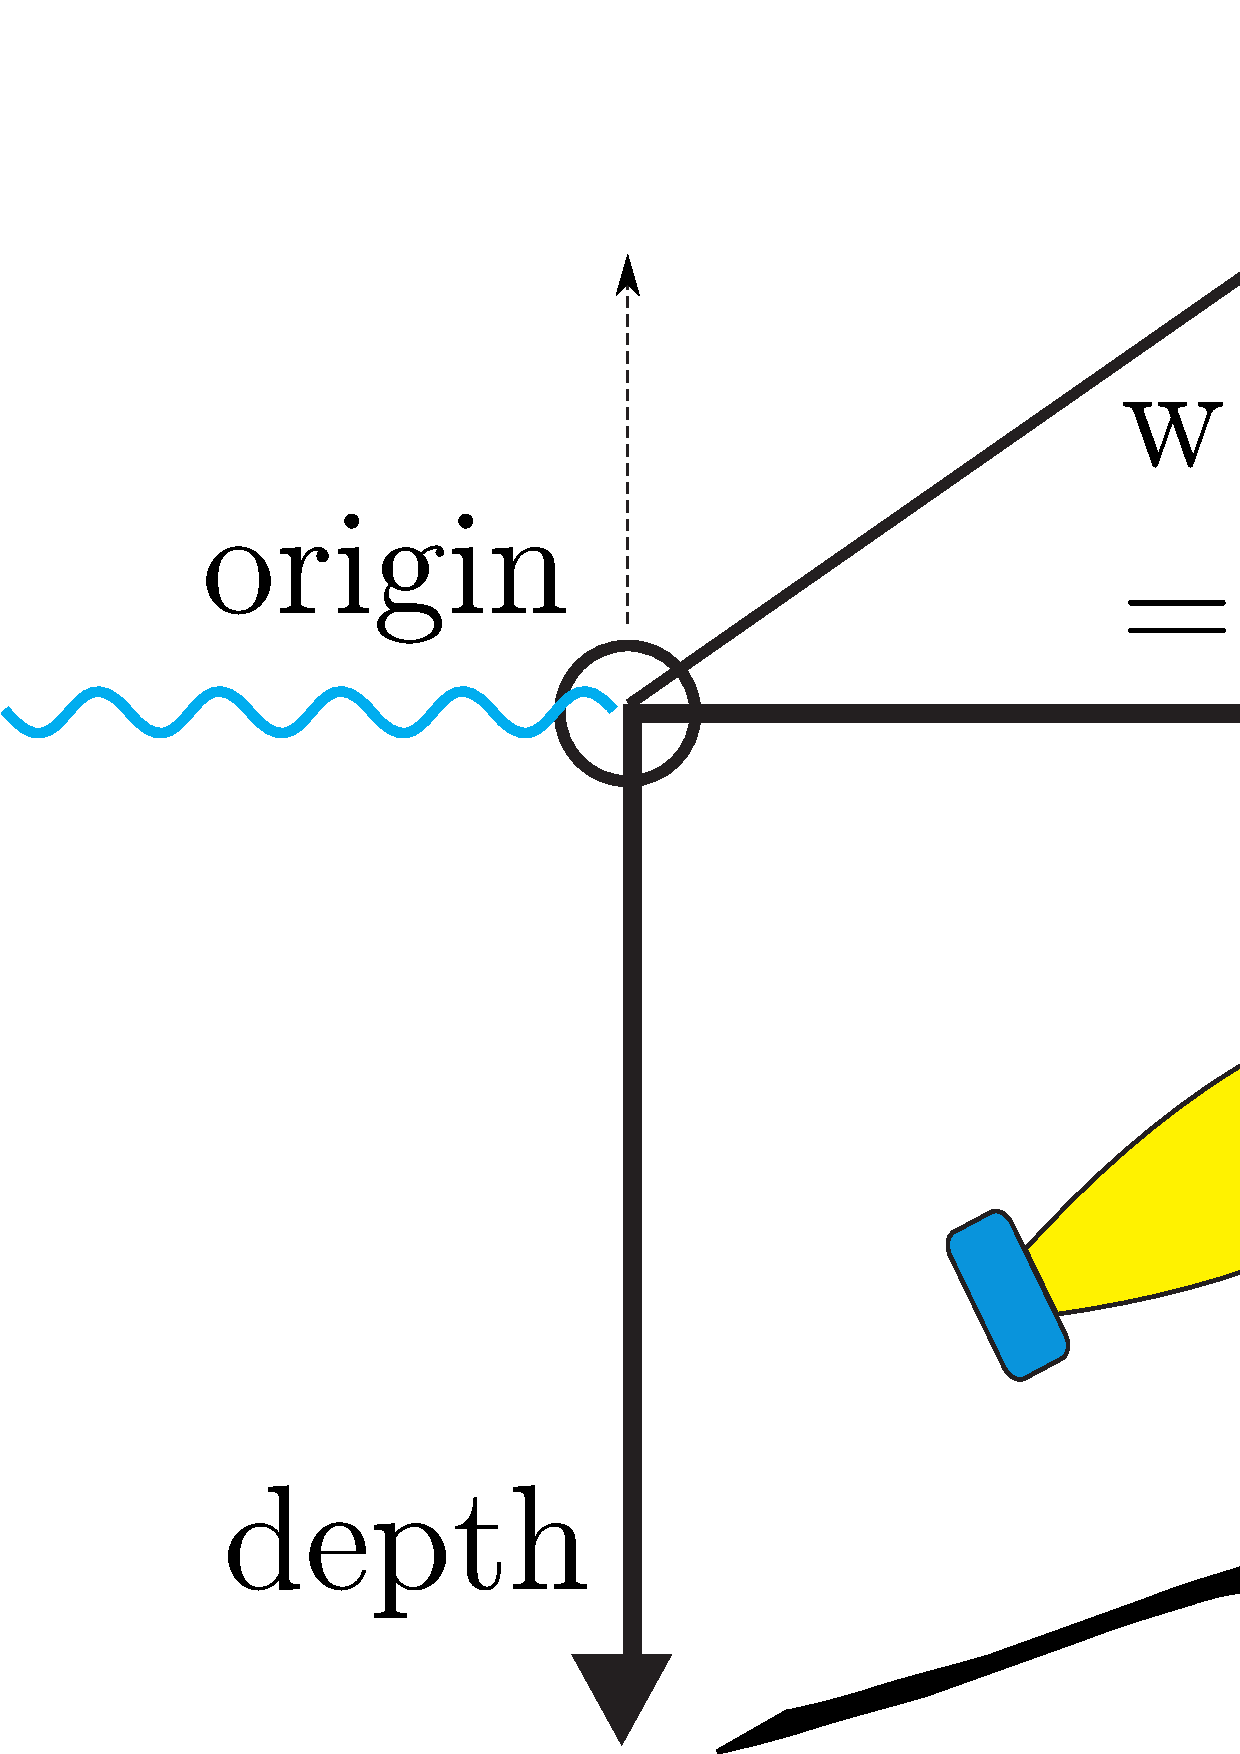
\includegraphics[width=0.48\linewidth]{auv-axes.pdf}
	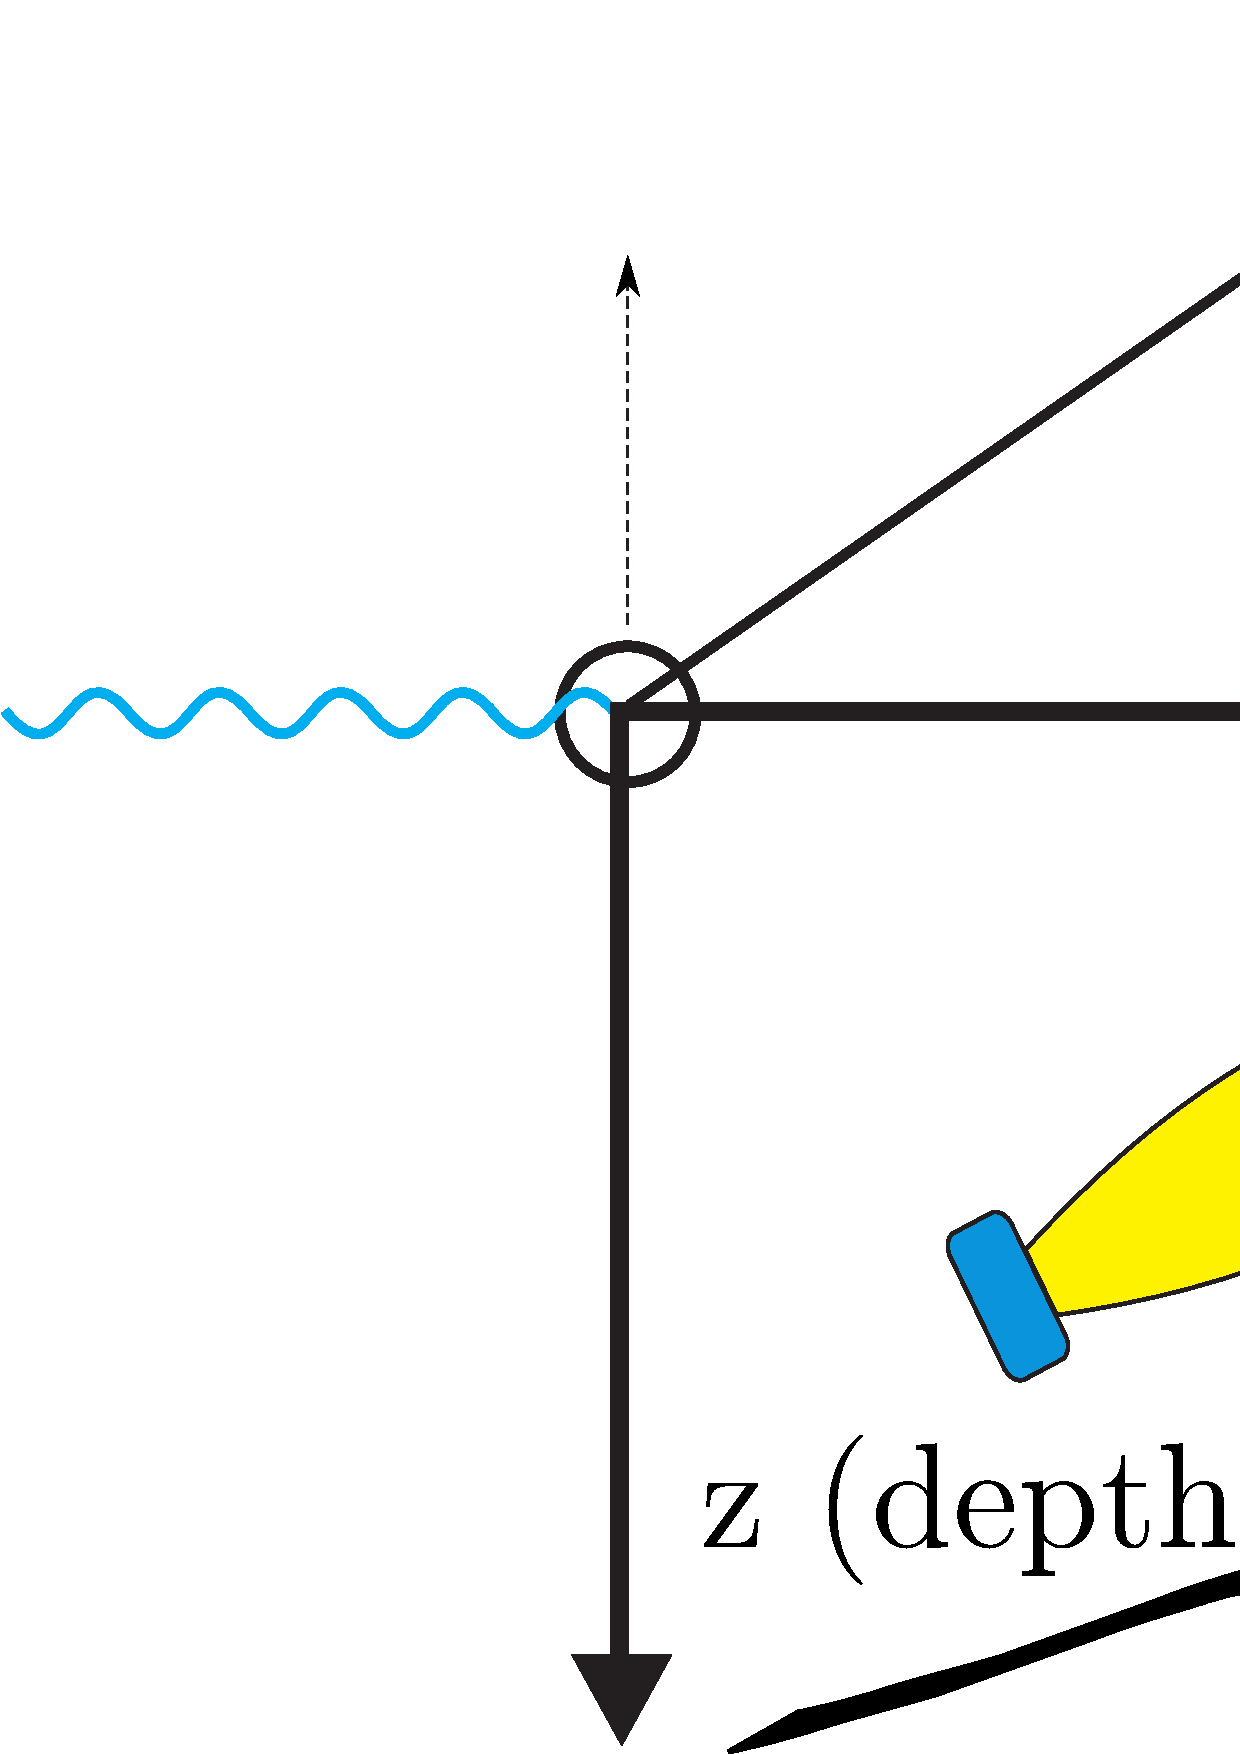
\includegraphics[width=0.48\linewidth]{auv-model.pdf}
\\	
	5 d.o.f. system model is describing how the state $\vect{X}(k)$ evolves in time. It is a \textit{constant speed} model \cite{ribas10} that uses previous state $\vect{X}(k-1)$ corrupted with zero-mean GRV acceleration noise to make a prediction of the next state vector value.
  \vspace{0.3em}
  }
%defined as
%%%%%%%%%%%%%%%%%%%%%%%%%%%%%%%%%%%%%%%%%%%%%%%%%%%%%%%%%%%%%%%%%%%%%%%%%%%%%%
  \headerbox{System model}{name=model,column=0,below=auv-navigation}{
%%%%%%%%%%%%%%%%%%%%%%%%%%%%%%%%%%%%%%%%%%%%%%%%%%%%%%%%%%%%%%%%%%%%%%%%%%%%%%
    A \textit{constant velocity} nonlinear model was used as a basis for the EKF state transition model.
\begin{equation}
\vspace{-5pt}
\vect{X}(k) = f(\vect{X}(k-1), \vect{N}(k-1))
\label{eq:state-tran}
\end{equation}
\begin{equation}
\begin{bmatrix} x \\ y \\ z \\ a \\ u \\ v \\ w \\ \psi \\ \varphi \\ \dot{\psi} \\ \dot{\varphi} \end{bmatrix}_{(k)} =
\begin{bmatrix} x + (uT+\dot{u}\frac{T^{2}}{2})\cos(\psi)\cos(\varphi) - (vT+\dot{v}\frac{T^{2}}{2})\sin(\psi)\cos(\varphi) \\ 
                y + (uT+\dot{u}\frac{T^{2}}{2})\sin(\psi)\cos(\varphi) + (vT+\dot{v}\frac{T^{2}}{2})\cos(\psi)\cos(\varphi) \\ 
                z + (wT+\dot{w}\frac{T^{2}}{2})\cos(\varphi) \\ 
                a - (wT+\dot{w}\frac{T^{2}}{2})\cos(\varphi) \\ 
                u + \dot{u}T \\ 
                v + \dot{v}T \\ 
                w + \dot{w}T \\ 
                \psi    + \dot{\psi}T    + \ddot{\psi}   \frac{T^{2}}{2} \\ 
                \varphi + \dot{\varphi}T + \ddot{\varphi}\frac{T^{2}}{2} \\ 
                \dot{\psi}    + \ddot{\psi}T \\ 
                \dot{\varphi} + \ddot{\varphi}T
\end{bmatrix}_{(k-1)} 
\label{eq:state-tran-matrix}
\end{equation} %% defined as zero-mean GRV.
	$\vect{N}(k) = \left[ \begin{array}{ccccc} \dot{u} & \dot{v} & \dot{w} & \ddot{\psi} & \ddot{\varphi} \end{array} \right]^{T}$ represents the process noise consisting of linear and angular accelerations. State vector elements are measured directly, hence measurement model $h()$ can be expressed with matrix containing ``ones'' at particular positions since the measurement relation becomes equality.
\begin{equation}
\vspace{-5pt}
\vect{Z}(k) = h(\vect{X}(k), \vect{M}(k)) = \vect{H} \vect{X}(k \mid k-1)  + \vect{M}(k)
\label{eq:mes-model}
\end{equation}
	$\vect{M}(k)$ is a zero-mean GRV vector representing the measurement noise. Measurement (observation) and process noise are characterised with diagonal covariation matrices whose elements $(\sigma_{N})$ are given as filtering parameters influencing estimation strategy.
  \vspace{0.3em}
  }
%available  
%%%%%%%%%%%%%%%%%%%%%%%%%%%%%%%%%%%%%%%%%%%%%%%%%%%%%%%%%%%%%%%%%%%%%%%%%%%%%%
  \headerbox{Sensor Fusion}{name=fusion,column=1,row=0}{
%%%%%%%%%%%%%%%%%%%%%%%%%%%%%%%%%%%%%%%%%%%%%%%%%%%%%%%%%%%%%%%%%%%%%%%%%%%%%%
	EKF implements sensor fusion. One of the features of navigation process is that sensor measurements are not available all the time. Simply - messages from sensors arrive at different moments and sensors could be unavailable due to different causes. The idea is to take all the gathered information at the moment of filtering and integrate it together in the measurement model (Eq. ~\ref{eq:fuse}), which varies depending on the measured values and sensors used for the measurement.
\\
    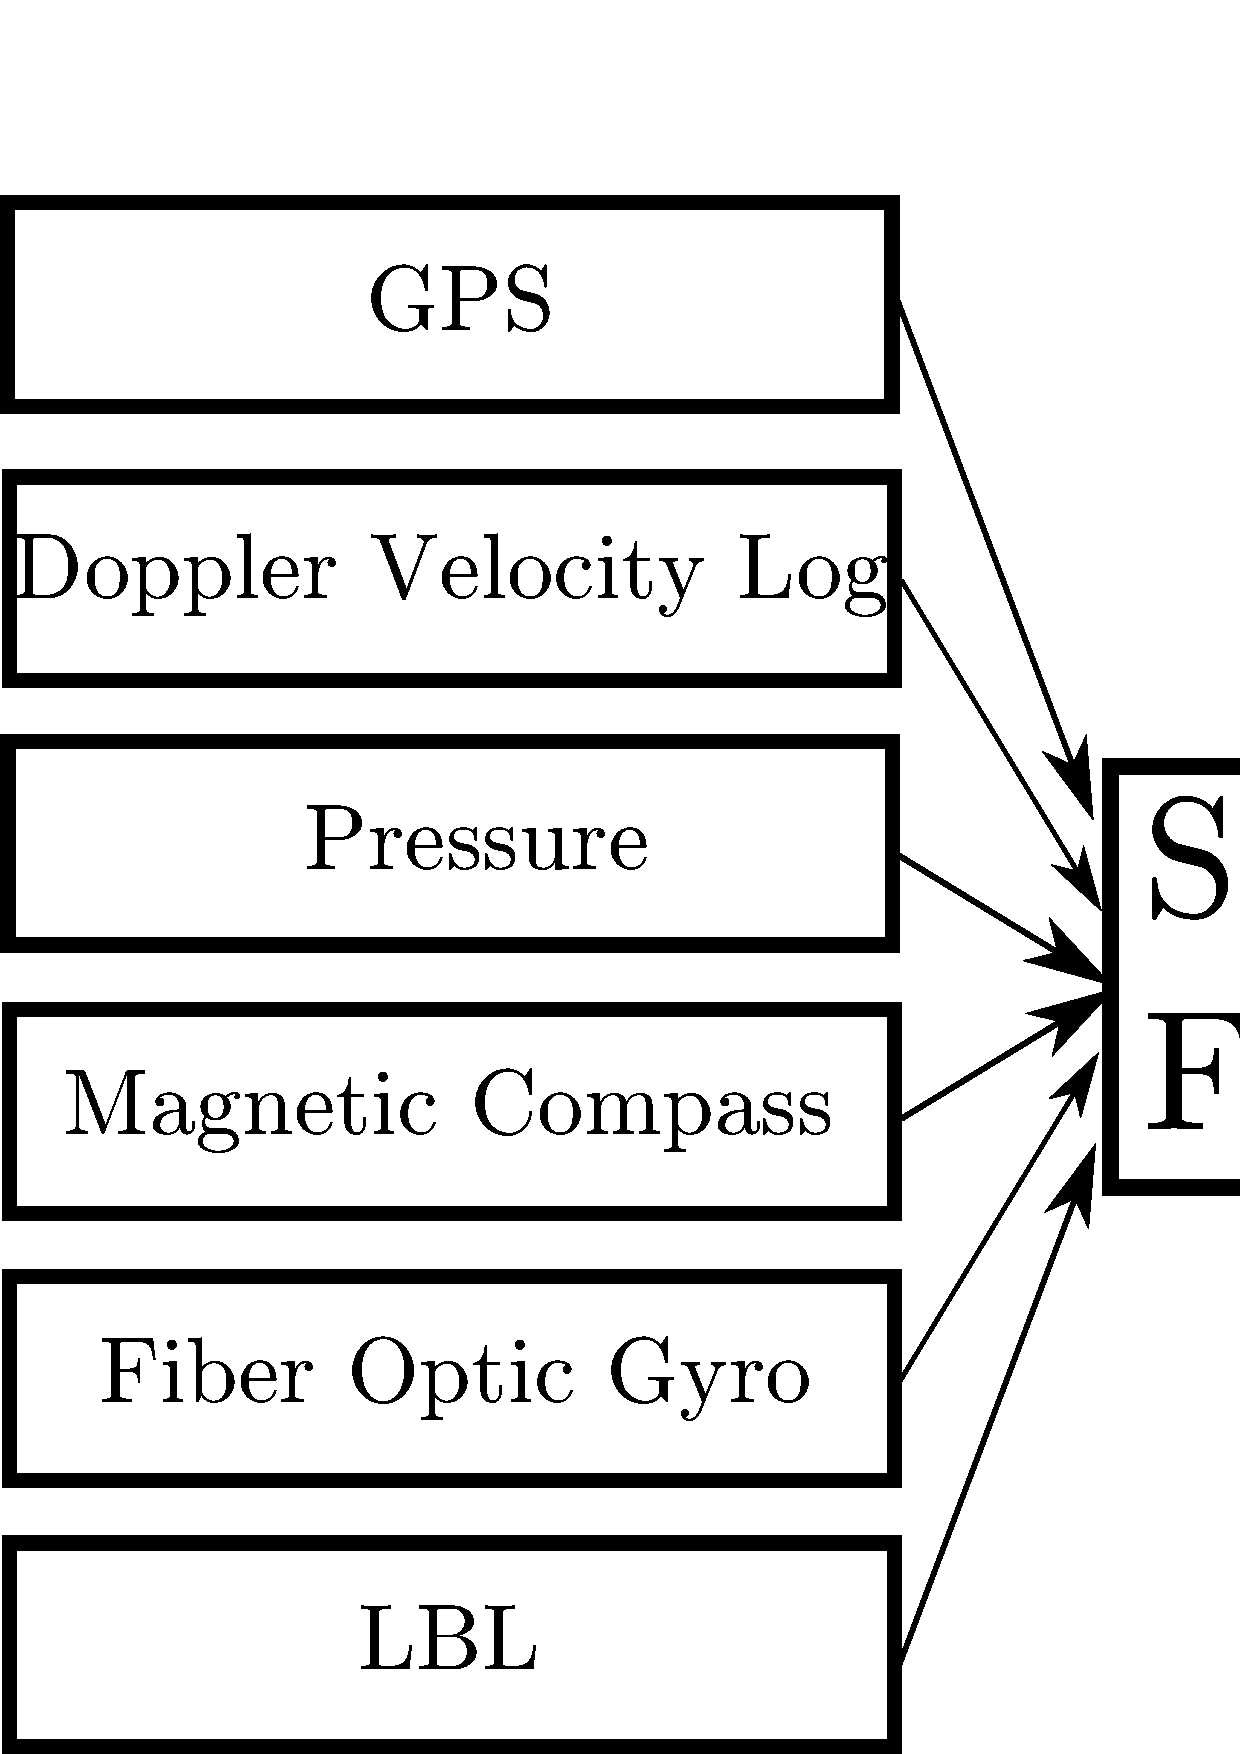
\includegraphics[width=0.97\linewidth]{fusion-all.pdf}
\\ \vspace{-25pt}
	\center{
	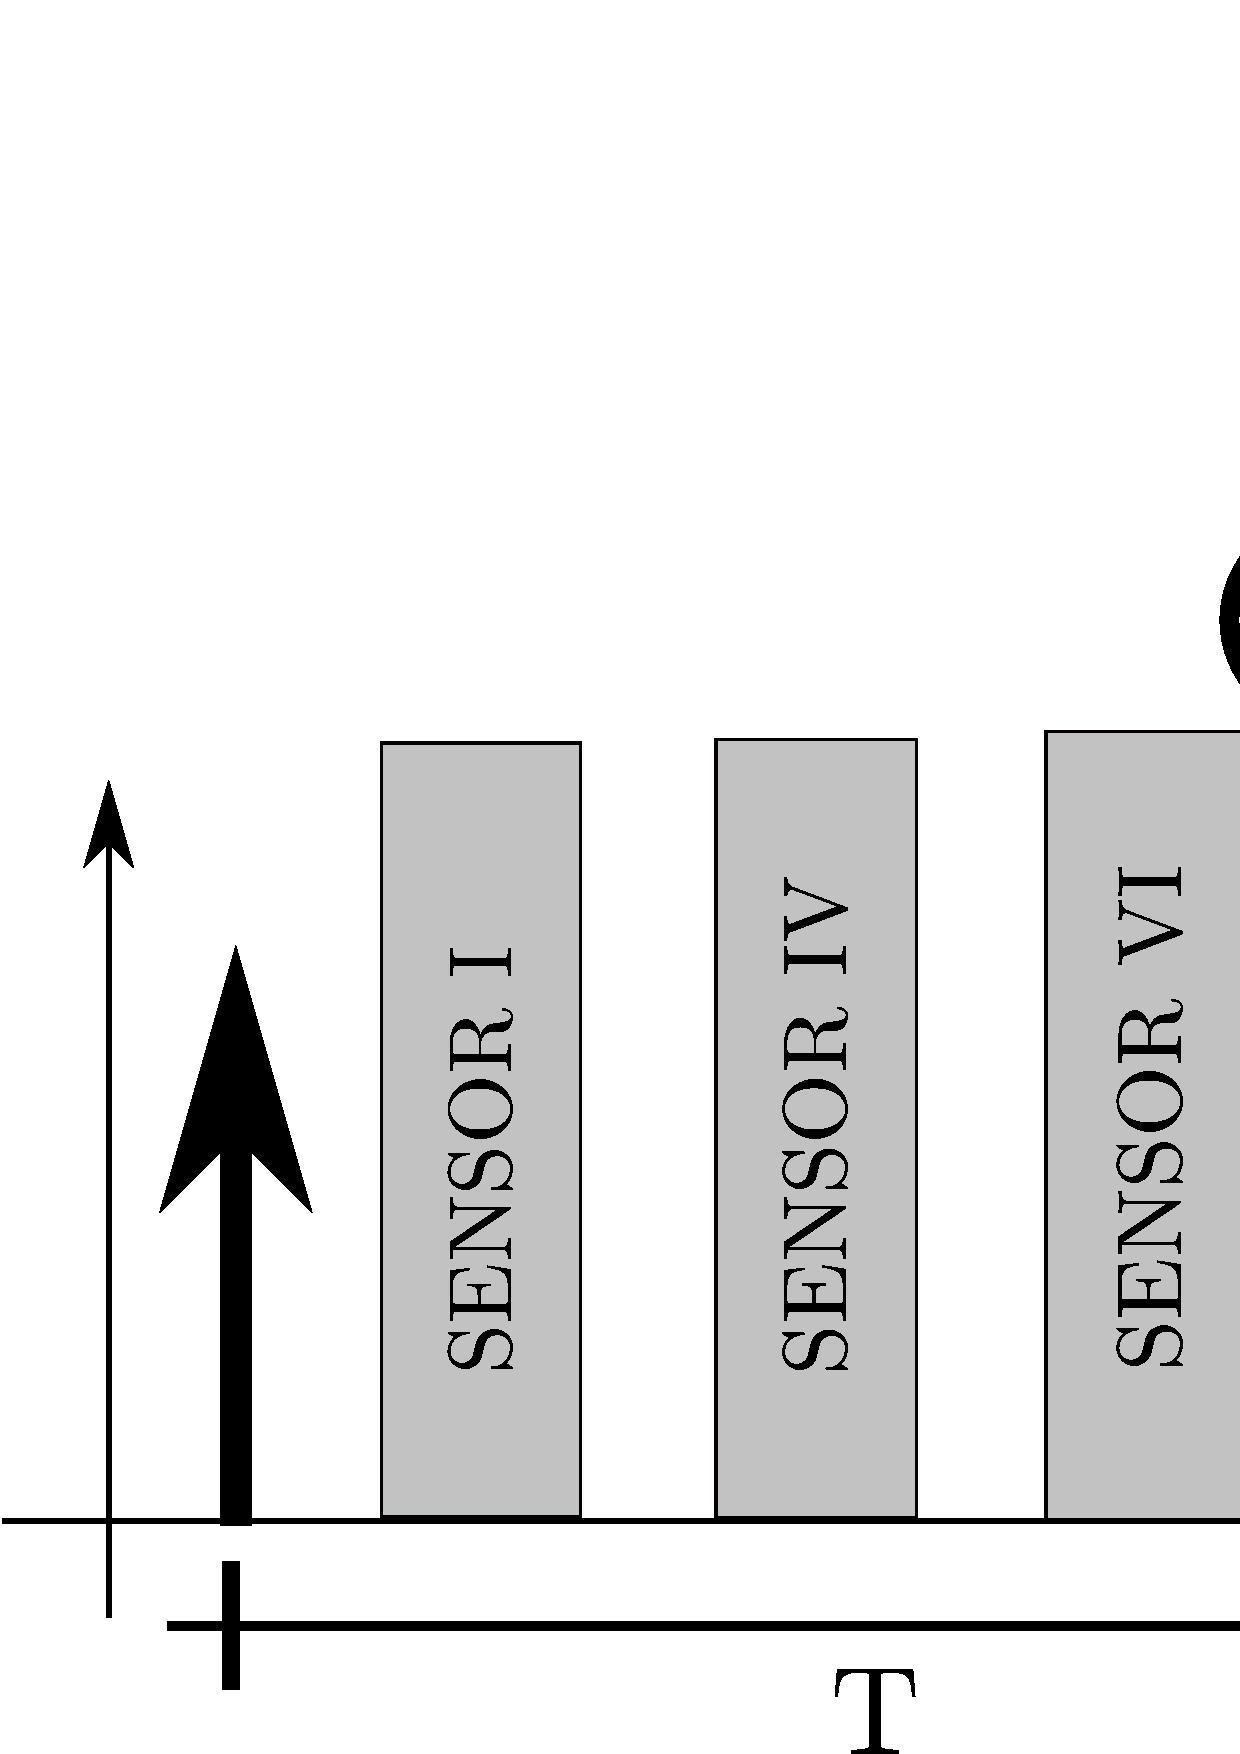
\includegraphics[width=0.53\linewidth]{synch.pdf}
	}
\\	
\vspace{-1em}
%sensor measurements included in observation. Kalman filter maintains its own timer. Observation is reset after each timer set period.  
\begin{equation}
\label{eq:fuse}
\vect{Z}(k) = \left[ \begin{array}{c} \vect{Z}_{sen. I} \\ \vect{Z}_{sen. II}  \end{array} \right],
\vect{H}(k) = \left[ \begin{array}{c} \vect{H}_{sen. I} \\ \vect{H}_{sen. II}  \end{array} \right], 
\vect{R}(k) = \left[ \begin{array}{ccc} \sigma_{sen. I}^{2} & 0 \\ 0 & \sigma_{sen. II}^{2} \end{array} \right]
\end{equation}	
  \vspace{-1.2em}
  }

%%%%%%%%%%%%%%%%%%%%%%%%%%%%%%%%%%%%%%%%%%%%%%%%%%%%%%%%%%%%%%%%%%%%%%%%%%%%%%
  \headerbox{Results}{name=results,column=1,below=fusion}{
%%%%%%%%%%%%%%%%%%%%%%%%%%%%%%%%%%%%%%%%%%%%%%%%%%%%%%%%%%%%%%%%%%%%%%%%%%%%%%
  \vspace{0.3em}
  Navigation method was tested on number of real missions with Nessie vehicle: 
  
$\bullet$ Spiral trajectory and surfacing action: localisation results in a smooth path, less prone to drifting than dead reckoning. EKF filters out the absolute position (LBL) outliers. Furthermore, sensor fusion is able to compensate for the missing measurements. Tuning of the filter parameters $(\sigma_{sen.})$ enables giving more or less trust in particular sensor measurements. Question of suitable choice of heading sensor can be treated by adjusting the trust given to \textit{yaw} and \textit{yaw rate} measurement obtained from different devices. 
\\
    {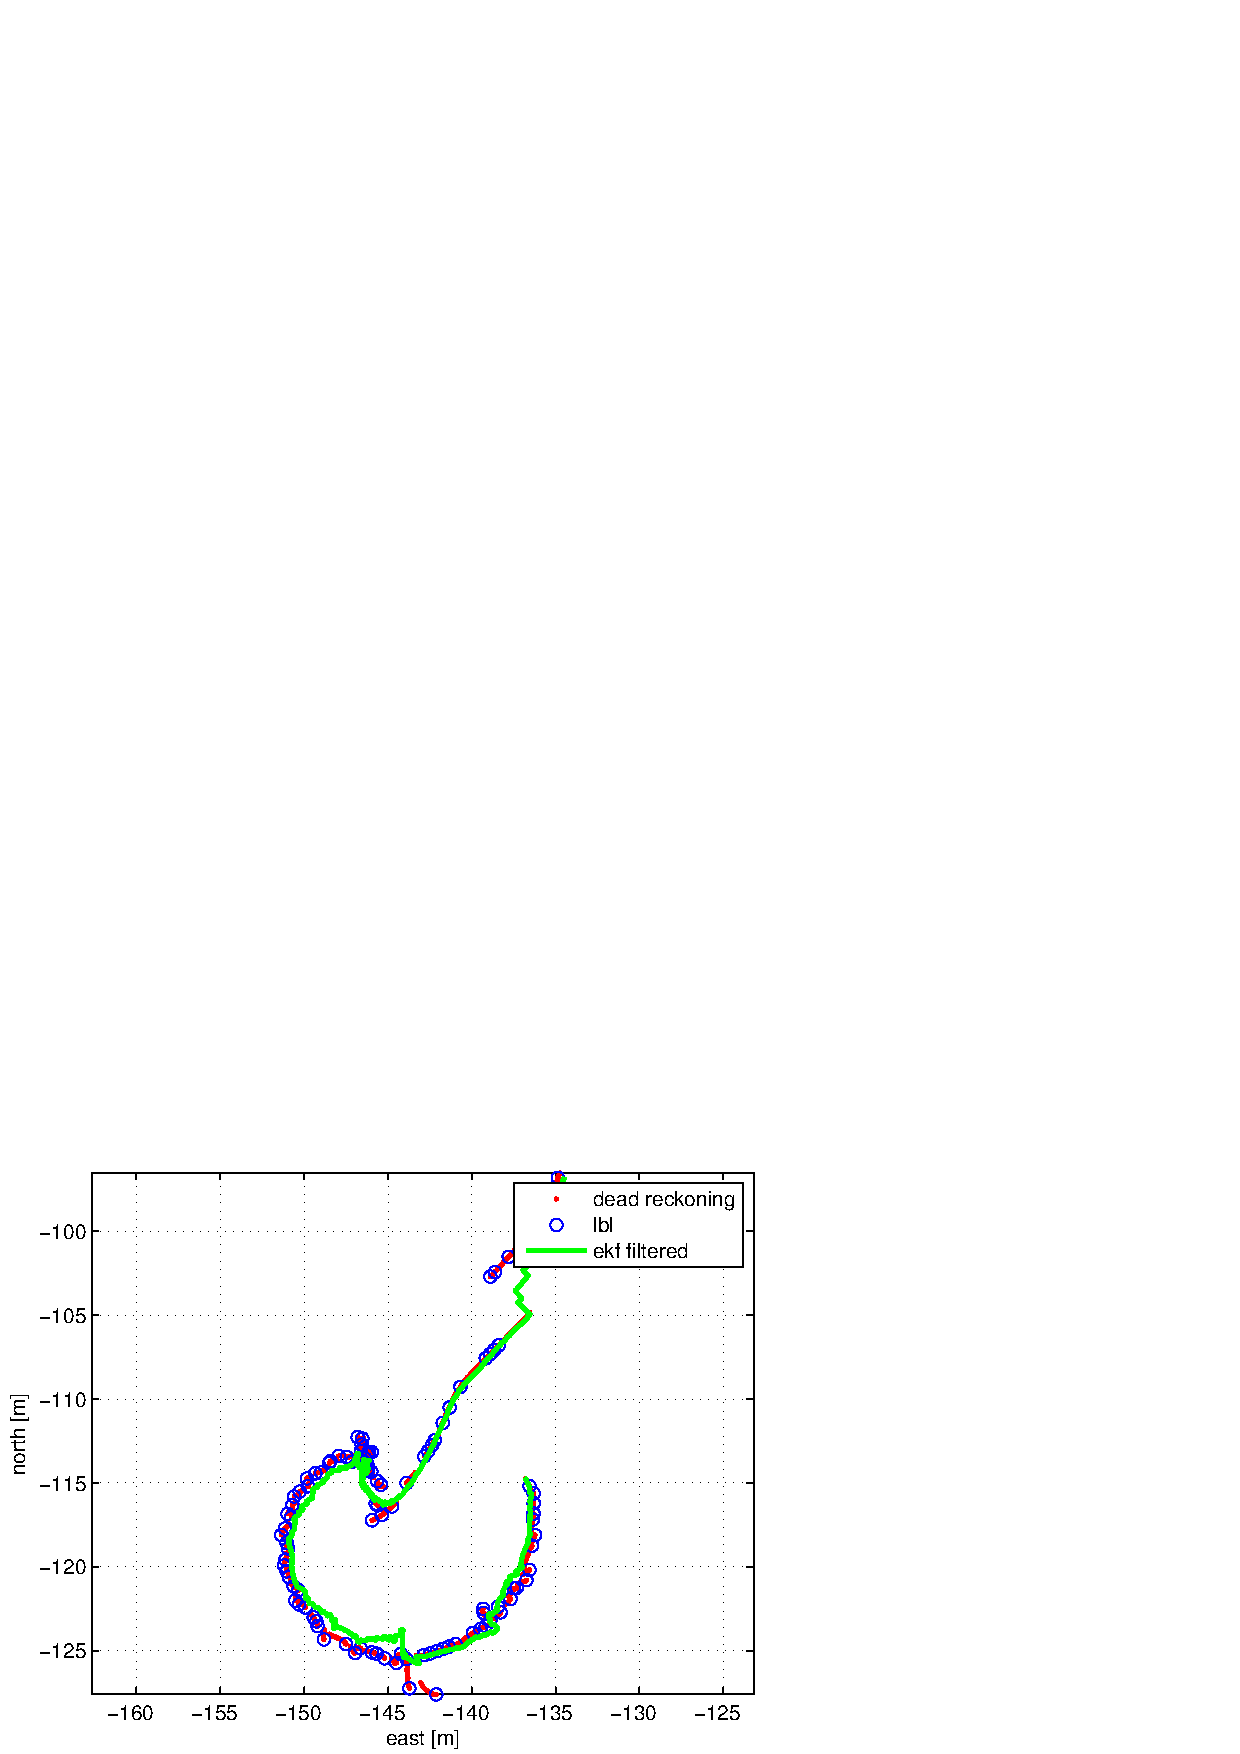
\includegraphics[width=0.5\linewidth]{spiral2d.pdf}}
	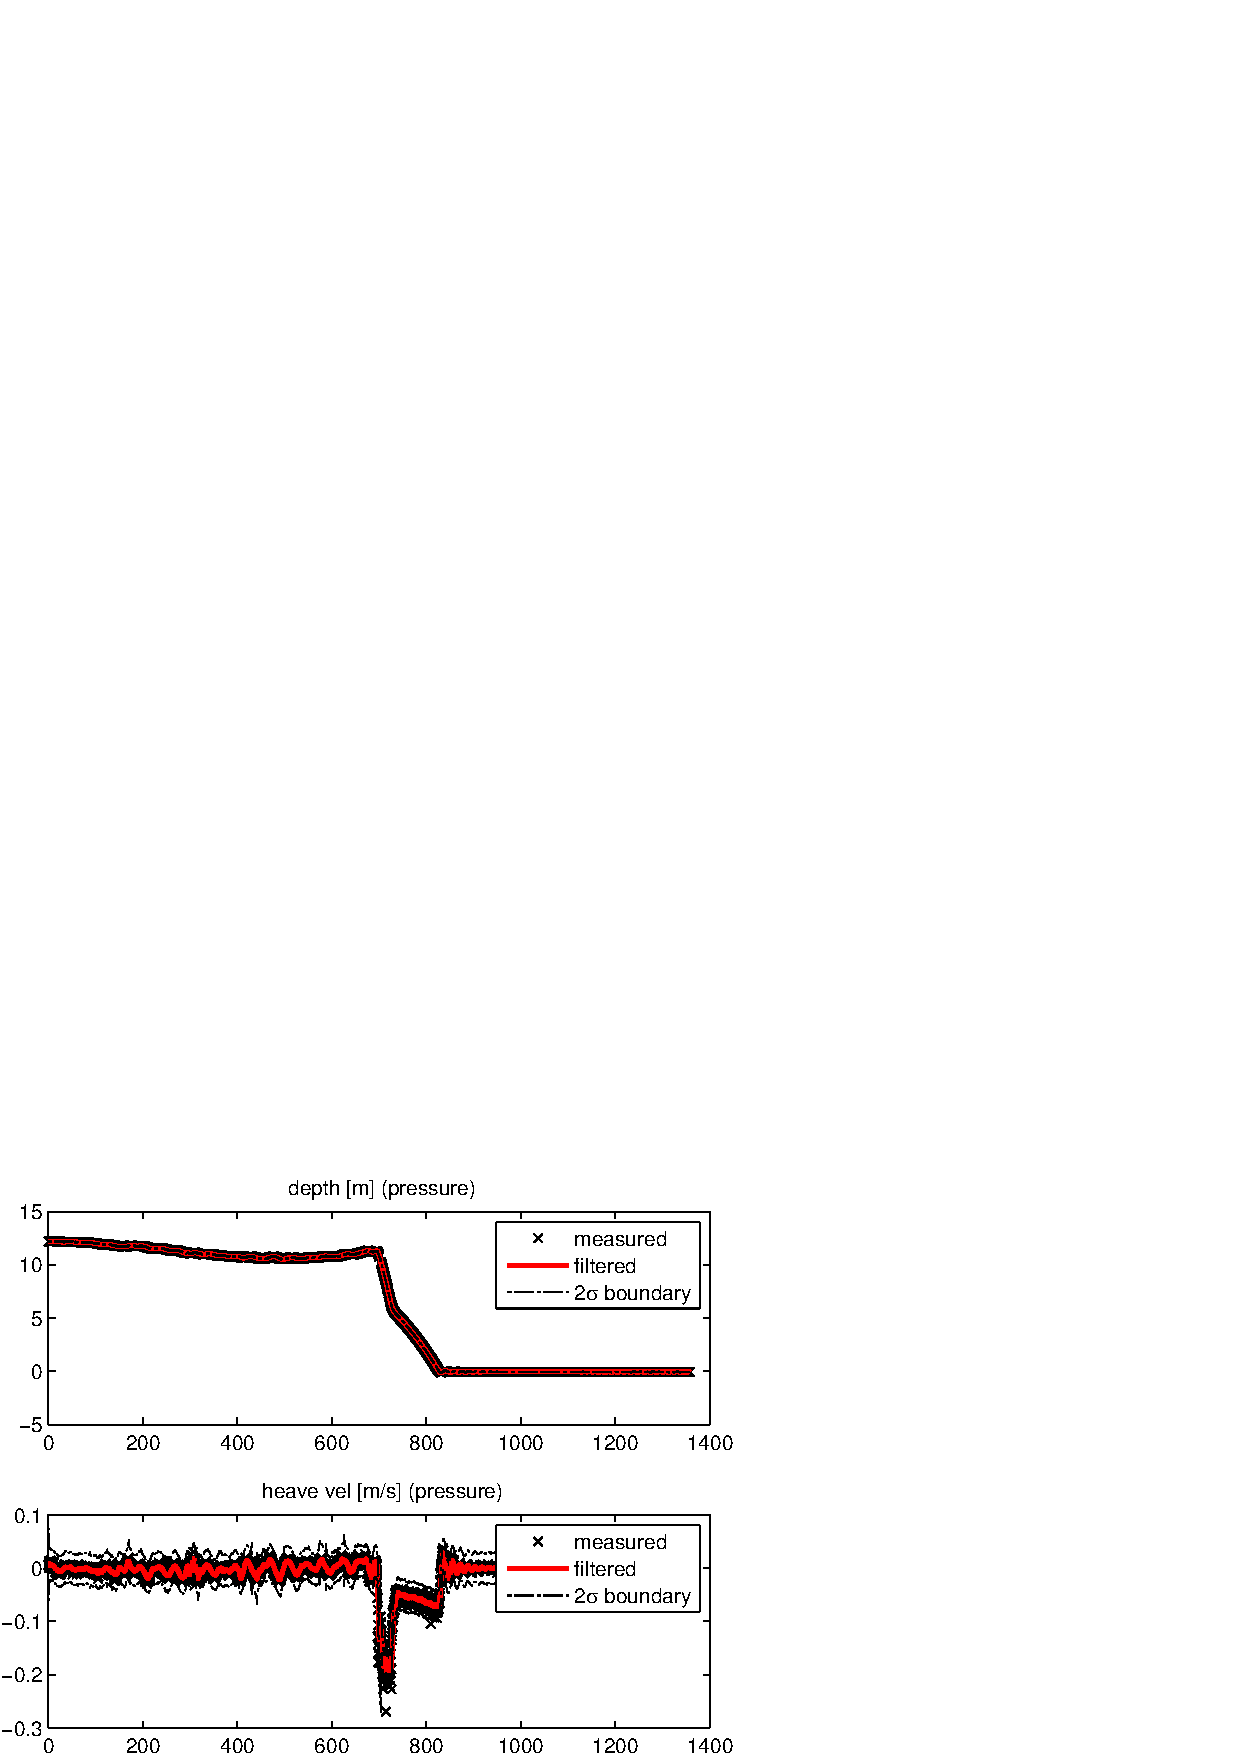
\includegraphics[width=0.43\linewidth]{spiral-depth.pdf}
\\	  
$\bullet$ Rectangular trajectory aided with GPS position measurements: localisation using Unscented Kalman Filter (UKF) was simulated using the real data. Trajectory obtained using UKF tends to be slightly more precise compared with the one obtained using EKF. 
\\	
\begin{tabular}{cl}
%\includegraphics[width=0.42\linewidth]{square.pdf}  &  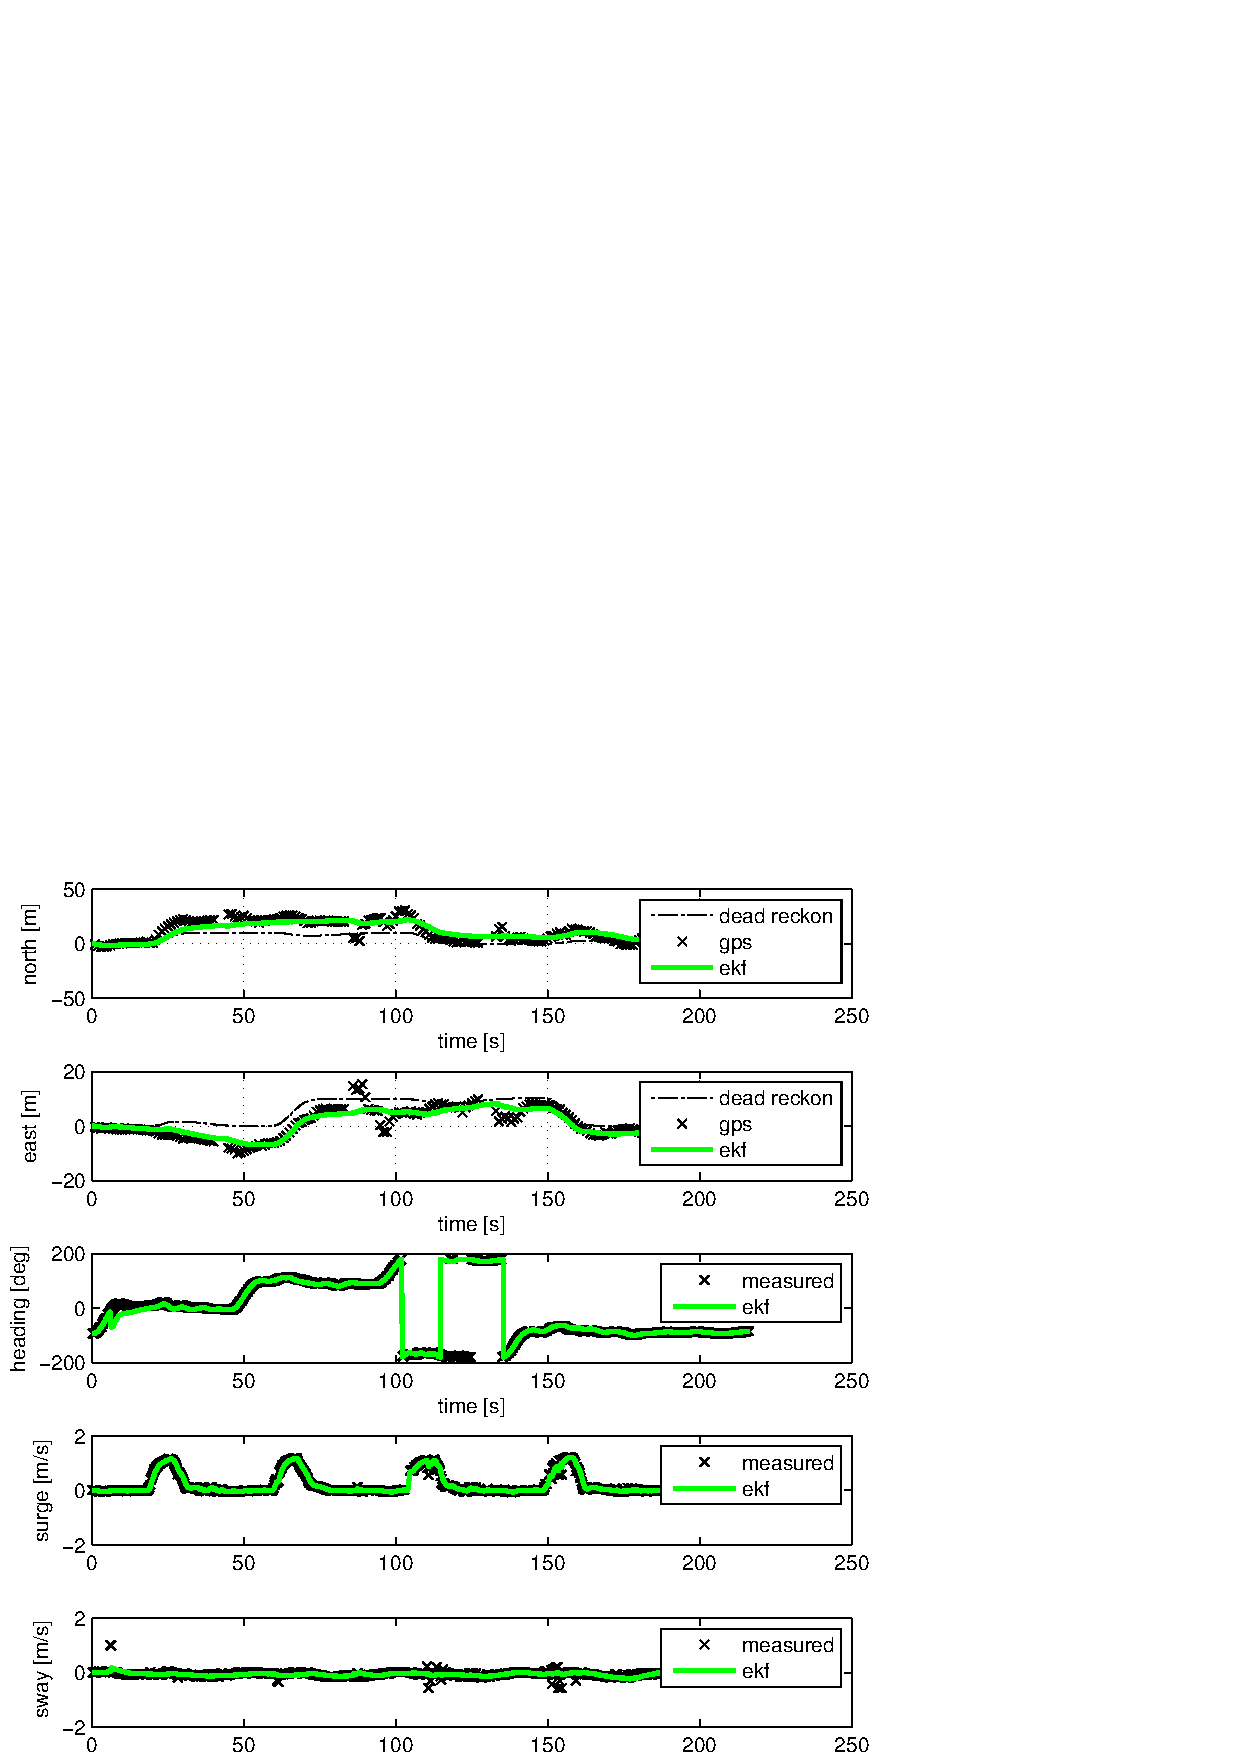
\includegraphics[width=0.54\linewidth]{square-filtering.pdf} \\
%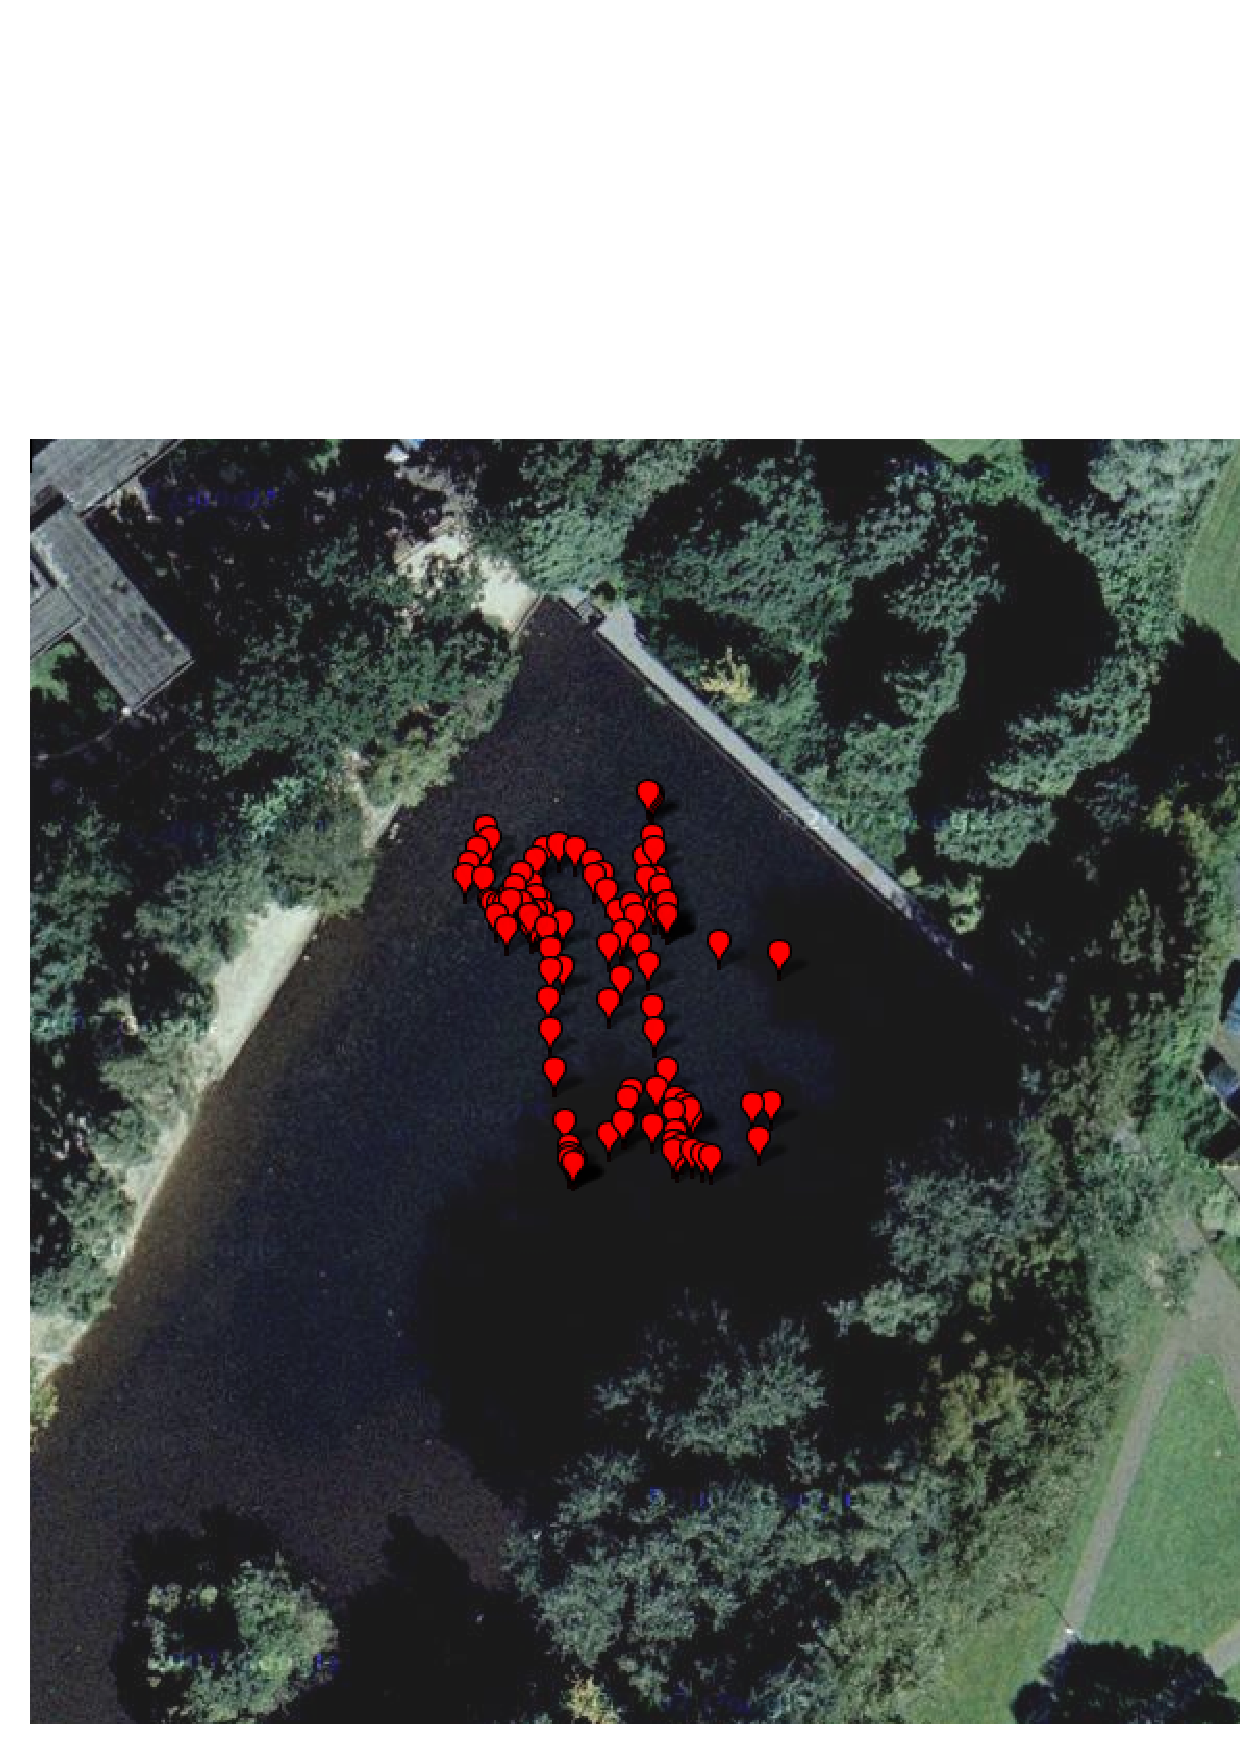
\includegraphics[width=0.3\linewidth]{square-trajectory.pdf} &   \\
\hspace{-1.0em} \includegraphics[width=0.4\linewidth]{square.pdf}             & \hspace{-1.0em} \multirow{2}{*}[9.8em]{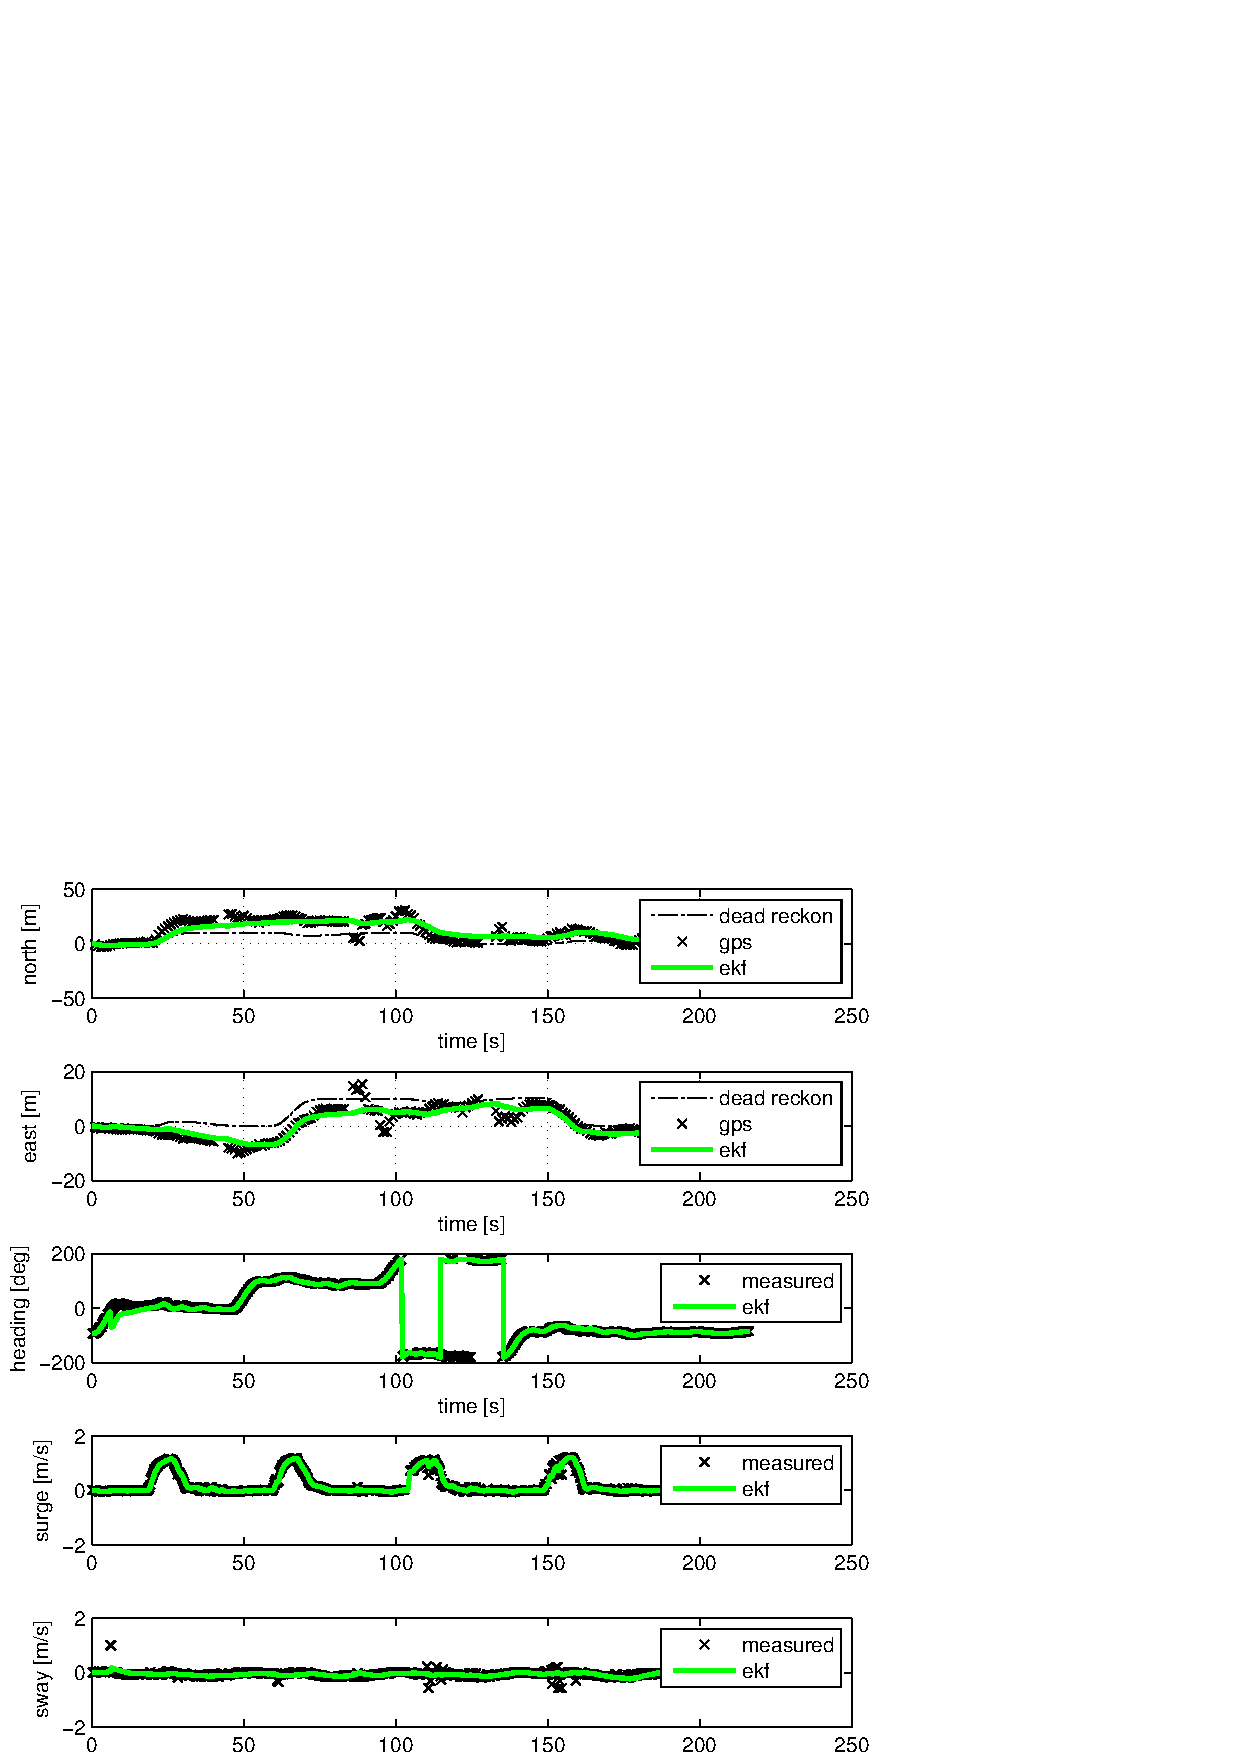
\includegraphics[width=0.56\linewidth]{square-filtering.pdf}} \\
\hspace{-1.0em} 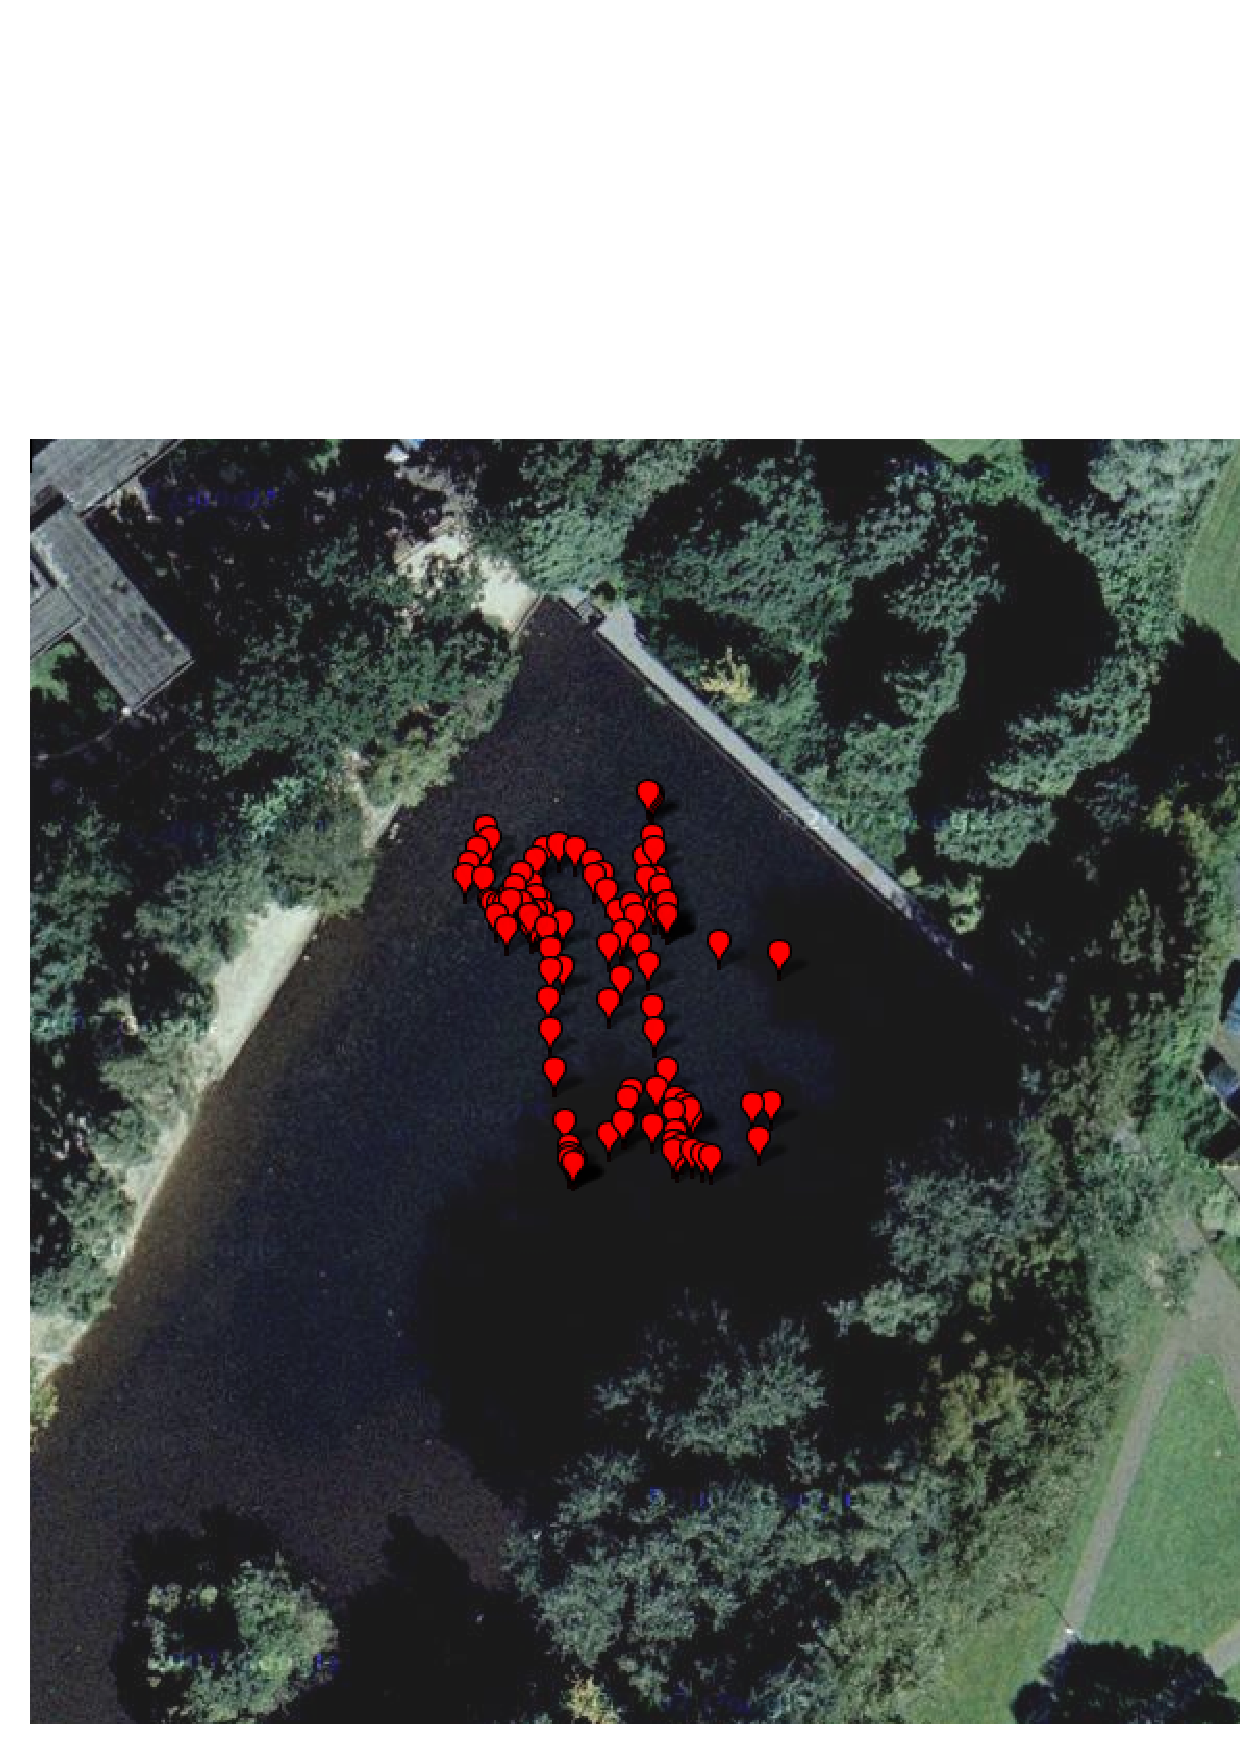
\includegraphics[width=0.23\linewidth]{square-trajectory.pdf} &  \hspace{-1.0em}   \\
\end{tabular}
EKF improves the localisation performance, even when confined to blend imprecise and sketchy position data from GPS.
  \vspace{0.3em}
  }

%%%%%%%%%%%%%%%%%%%%%%%%%%%%%%%%%%%%%%%%%%%%%%%%%%%%%%%%%%%%%%%%%%%%%%%%%%%
  \headerbox{References}{name=references,column=0,span=2,above=bottom}{
%%%%%%%%%%%%%%%%%%%%%%%%%%%%%%%%%%%%%%%%%%%%%%%%%%%%%%%%%%%%%%%%%%%%%%%%%%%  
    \smaller
    \vspace{-0.6em} %\hspace{4.5em}
    \bibliographystyle{ieee}
    \renewcommand{\section}[2]{\vskip 0.05em}
      \begin{thebibliography}{1}\itemsep=0.05em
      \setlength{\baselineskip}{0.1em}
      \bibitem{ribas10} 
      D. Ribas, P. Ridao, and J. Neira.
      \newblock {U}nderwater {S}lam for {S}tructured {E}nvironments using an {I}maging {S}onar
      \newblock {\em Springer Verlag, 2010}
      \bibitem{thrun05}
      S. Thrun, W. Burgard, and D. Fox.
      \newblock {P}robabilistic robotics
	  \newblock {\em MIT Press, 2005}	      
      %\bibitem{ristic04}
      %B. Ristic, S. Arulampalam, and N. Gordon.
      %\newblock {B}eyond the {K}alman filter {P}article filters for tracking applications
	  %\newblock {\em Artech House Publishers, 2004}
      \end{thebibliography}
      %\vspace{0.01em}
  }
\end{poster}

\end{document}
